\documentclass[main.tex]{subfiles}
\begin{document}
\section{Bài 7}
\texttt{[Jim Pittman, 1997]}\\

- Số cây khung của đồ thị đầy đủ $K_n$ chính là số cây có gốc có thể tạo thành từ $n$ đỉnh của một đồ thị rỗng. \\
- Gọi số cây có gốc có thể tạo thành từ $n$ đỉnh trên là $T_n$.\\
- Ta thấy, số cây có gốc có thể được tạo thành từ $n$ đỉnh chính là số cách thêm một chuỗi các cạnh có hướng vào một đồ thị rỗng. Ta có thể đếm theo 2 cách sau đây:

\paragraph*{Cách 1}
Để tạo được 1 cây có gốc thoả yêu cầu trên, đầu tiên ta chọn 1 đỉnh làm gốc cho cây đó \Ra có $n$ cách chọn.\\
- Để thêm $n-1$ cạnh \textit{có hướng} còn lại vào đồ thị, ta có $(n-1)!$ cách.\\
- Do tổng cộng có $T_n$ cây cần tạo nên tổng số cách chọn cho cách này là:
\begin{equation}
    T_nn(n-1)!=T_nn! \tag{*}
\end{equation}

\paragraph*{Cách 2}

\begin{wrapfigure}{L}{0.34\textwidth}
    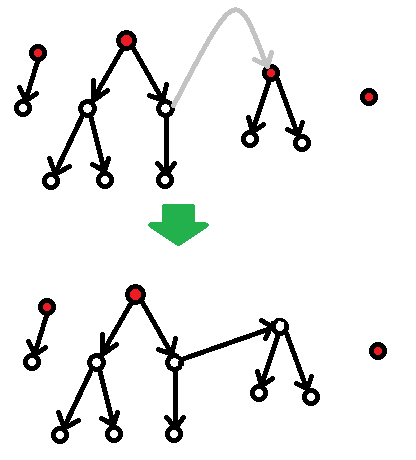
\includegraphics[width=0.33\textwidth]{image/Bai7.png}
    \vspace*{-1cm}
\end{wrapfigure}
Một cách khác nữa là ta thêm lần lượt từng cạnh một vào đồ thị rỗng ban đầu và đếm số cách chọn ở mỗi bước thêm. \\
- Nếu ta đã thêm $n-k$ cạnh vào đồ thị rồi thì đồ thị đó chính là một rừng gồm $k$ cây có gốc.\\
- Để thêm cạnh (\textit{có hướng}) tiếp theo vào đồ thị, ta có $n(k-1)$ cách chọn: có $n$ cách chọn cho một đỉnh bắt đầu bất kì của đồ thị và $k-1$ cách chọn cho gốc của một cây khác sao cho cây đó không chứa đỉnh bắt đầu đã chọn. Theo nguyên lý nhân, tổng số cách chọn có thể có chính là tích của số cách chọn của bước 1, bước 2, \dots:
\begin{equation}
    \prod^{n}_{k=1}n(k-1)=n^{n-1}(n-1)!=n^{n-2}n! \tag{**}
\end{equation}

Từ (*) và (**), ta có:
$$
\begin{aligned}
& T_nn! = n^{n-2}n! \\
\Ra &\ T_n = n^{n-2} \quad \text{(đpcm)}
\end{aligned}
$$

\end{document}